\section{Related Work}

A  \emph{generalized permutahedron} in $\RR^n$ is a convex polytope such that all its edges are parallel to $e_i-e_j$ for $i\neq j$. \newline Here $e_1,e_2,\dots,e_n$ denote the standard "jdkjdfkjg. shfiui. " basis vectors of $\RR^n$. \\ Generalized permutahedra were introduced by Postnikov \cite{Postnikov:2009}, but they were known before under different names, most notably in the context of submodular function optimization~\cite{Fujishige:2005, Murota:2003} and discrete convex analysis~\cite{Murota:2003}. 
Relevant examples of generalized permutahedra Chr. include the regular permutahedra, Bruhat interval polytopes, hypersimplices and more general matroid polytopes. 
\paragraph{test}
In this way the topic is connected to group and representation theory, algebraic and tropical geometry, optimization and beyond.

Here we initiate the combinatorial study of polyhedral subdivisions of generalized permutahedra into cells which are again generalized permutahedra.
We call these \emph{permutahedral subdivisions}.
An important special case are the tropical linear spaces, which amount to regular subdivisions of matroid polytopes with matroidal cells; see \cite[\S4.4]{Tropical+Book} and \cite[\S10.5]{ETC}. \n Our first main contribution (\Cref{thm:regular-2-skeleton}) is a description of regular permutahedral subdivisions of the regular permutahedra in terms of conditions on the $2$-skeleton. \newline This result is an adaptation of the characterization of the uniform tropical linear spaces via the $3$-term Plücker relations.

One motivation for research in this direction comes from the wish to understand flags of tropical linear spaces and flag matroids. As a new tool, we prove a characterization of pairs of valuated matroids in terms of tropical incidence relations (\Cref{thm:1step}). 
Speyer and Williams~\cite{SpeyerWilliams:2021} and, independently, Arkani-Hamed, Lam, and Spradlin \cite{ArkaniHamedLamSpradlin:2021} recently showed that the positive Dressian equals the positive tropical Grassmannian. \\ Our second main result (\Cref{thm:positivity}) is related, as it shows that the valuated flags which can be realized by a totally positive flag of linear spaces correspond to the permutahedral subdivisions whose cells are Bruhat interval polytopes.

\acknowledgements
We want to thank Daniel Corey and Ben Smith for their feedback and Lauren Williams for pointing us to~\cite{Boretsky:2021} and for sharing insights regarding Bruhat interval polytopes.


% We call the resulting subdivision \emph{M-convex}, too. MJ: Does not make sense as we already introduced "permutahedral".

%% A \emph{valuated g-permutahedron} is a pair $(P,w)$ where $P$ is a generalized permutahedron and $w$ is a height function defined on the vertices.
%% That is a \emph{valuated permutahedron} if $P$ is the regular permutahedron $\Pi_n$.

% \begin{itemize}
	% \item \emph{g-permutahedron} = generalized permutahedron
	% \end{itemize}




% \begin{example}
	%   Let $M$ be a matroid on $n$ elements of rank $d$.
	%   We can identifying the bases of $M$ with $0/1$-vectors of length $n$ with exactly $d$ ones; i.e., with vertices of the hypersimplex $\Delta(d,n)$.
	%   Taking their convex hull we obtain a polytope $P(M)$, the \emph{matroid (base) polytope} of $M$.
	%   By construction $P(M)$ is a subpolytope of $\Delta(d,n)$, and it is a block thanks to \cite{GelfandEtAl87}; see also \cite[Theorem 10.36]{ETC}.
	%   From the same result it follows that the matroid subdivisions of $\Delta(d,n)$, i.e., the polyhedral subdivisions where each cell is a matroid polytope, are precisely the block subdivisions of $\Delta(d,n)$.
	% \end{example}


\section{Geometry of the regular permutahedron}
\label{sec:geometry-regular-permutahedron}

We denote the symmetric group of degree $n$ as $\Sym(n)$.
The (regular) permutahedron $\Pi_n\subseteq \RR^n$ is defined as the convex hull of the points $(\sigma(1),\sigma(2),\dots,\sigma(n))$, where $\sigma$ ranges over $\Sym(n)$. 
These points form the $n!$ vertices of $\Pi_n$, and $\Sym(n)$ acts on this set, e.g., by multiplication on the right.
We have $\dim\Pi_n=n-1$.
Throughout, we identify $\Sym(n)$ with the vertices of $\Pi_n$. 

The face structure of $\Pi_n$ is well-known, and we will use the following description.
A \emph{flag} $(F_1,\dots,F_k)$ in $[n]$ with $k$ \emph{constituents} is a strictly increasing sequence $F_{1}\subset \dots \subset F_{k}$ of non-empty subsets of $[n]$; a flag is \emph{full} if it has $n$ constituents.
We say that a flag \emph{extends} a pair $(U,V)$ of subsets $U \subset V \subseteq [n]$ if there are $i,j \in [k]$ with $U = F_i$ and $V = F_j$.
We set $e_A:= \sum_{i\in A} e_i$.
For the flag $\cF=(F_1,\dots,F_k)$ we can pick real numbers $\lambda_i$ with $\lambda_1 \gg \dots \gg \lambda_k> 0$ to obtain the vector 
\[
\lambda_\cF := \lambda_1 e_{F_1} +\lambda_2 e_{F_2\backslash F_1} +\dots +\lambda_ke_{F_k\backslash F_{k-1}} \, .
\]
The following summarizes results from \cite[Section 3.3(d)]{Fujishige:2005} and \cite[Proposition 1.3]{BilleraSarangarajan:1996}.
%A \emph{jump} of $\cF$ is a pair of subsequent constituents $(F_{k-1},F_k)$ such that $F_k\setminus F_{k-1}$ contains more than one element; here we use the convention $F_0=\emptyset$ and $F_n=[n]$.
\begin{proposition} \label{faces-permutahedron}
	The map which sends the flag $\cF=(F_1,\dots,F_k)$ in $[n]$ to the non-empty proper face of $\Pi_n$ which maximizes $\lambda_\cF$ is a bijection.
	In particular,
	\begin{compactenum}
		\item the flag $\cF$ with $k$ constituents corresponds to a face of codimension $k$, which is affinely equivalent with $\Pi_{|F_1|} \times \Pi_{|F_2 \setminus F_1|} \times \dots \times \Pi_{|F_k \setminus F_{k-1}|} \times \Pi_{|[n] \setminus F_k|}$;
		\item the facets correspond to non-empty proper subsets of $[n]$;
		\item the vertices correspond to the full flags;
		\item the edges correspond to pairs of full flags which differ in exactly one constituent;
		\item each $2$-face, where $k=n-3$, is either a hexagon (if there exists $i$ with $|F_{i+1} \setminus F_i| = 3$), or it is a square (if there exist distinct $i,j$ with $|F_{i+1} \setminus F_i| = 2$ and $|F_{j+1} \setminus F_j| = 2$).
		\item for two sets $A,B \subset [n]$ with $|A| = |B|$ and $|A \triangle B| = 2$, the edges defined by the flags extending $(A \cap B, A \cup B)$ span a face isomorphic with $\Pi_{|A \cap B|} \times \Pi_{2} \times \Pi_{n - |A \cup B|}$.
	\end{compactenum}
\end{proposition}
Here, '$\triangle$' denotes symmetric difference. 
Notice that $\Pi_n$ also arises as a secondary polytope of the prism over an $(n{-}1)$-simplex; see \cite[Theorem 6.2.6]{Triangulations}.
This leads to another way to describe the face lattice.
% number of $k$-faces = OEIS:A019538


\section{Flag matroids and subpermutahedra}

%% \begin{enumerate}
	%% 	\item $\{2,4,13,24\}$,  8 vertices, 24 members. %$A1A1A1B2$ $[b,e,f]$ 
	%% 	\item $\{3,4,34,124\}$,  8 vertices, 12 members. 	%$A1A1B1B2$ $[a,d,e]$
	%% 	\item $\{3,4,23,13,34\}$, 8 vertices, 24 members.	%$A1A2$		$[a,e,f]$
	%% 	\item $\{4,14,23,24,34,234\}$, 8 vertices, 12 members.	%$A2A2$   $\CC[a,b,d,f]/(ad-b)$
	%% 	\item $\{3,4,34,134,234\}$, 8 vertices, 6 members.	%$B3$	$\CC[a,d,e,f]/(df-e)$
	%% 	\item $\{4,13,234\}$, 10 vertices, 24 members. %$A1A1B1$ $\CC[a,b,e,f]/(ae+bf)$
	%% 	\item $\{3,4,34\}$, 12 vertices, 12 members. %$A1A1B2$
	%% 	\item $\{4,14,24,34\}$, 12 vertices, 8 members. %$A2$
	%% 	\item $\{124,3\}$, 12 vertices, 4 members. %(opposite faces) $A1A1a$
	%% 	\item $\{4,234\}$, 14 vertices, 12 members. %(non-opposite faces) $A1A1b$
	%% 	\item $\{4,23\}$, 14 vertices, 24 members. %$A1B1$
	%% 	\item $\{14,23\}$, 16 vertices, 3 members. %$B1B1$
	%% 	\item $\{4\}$, 18 vertices, 8 members. %$A1$
	%% 	\item $\{34\}$ 20 vertices, 6 members. %$B1$
	%% 	\item $\emtpyset$ 24 vertices, 1 member. %$\Pi_n$
	%% \end{enumerate}%Old labeling in comment


%\begin{definition}
%A {\it flag} $F$ on $[n]$ is a strictly increasing sequence $F_{1}\subset .... \subset F_{k}$ such that $F_{i}\subseteq [n]$ for all $i\in [k]$. 
%The {\it rank} of $F$ is the tuple $(r_{1},...,r_{k})$, where $r_{i}$ is the cardinality of $F_{i}$. 
%We call $F_{i}$ the ith {\it constituent} of $F$.
%\end{definition}

%% \begin{itemize}
	%% \item Definition of valuated matroid
	%% \item matroid (in terms of bases / polytope)
	%% \item Example
	%% \item Put valuated matroid quotient + Remark
	%% \item Matroid quotient, Flag matroid, flag matroid base polytope
	%% \item Theorem by GBW
	%% \item Bruhat interval polytopes
	%% \item  Valuated permutahedra
	%% \item Valuated flag
	%% \item Compression / convolution
	%% \item Theorem by BEZ
	%% \item Move Theorem on incidence relations up 
	%% \end{itemize}

\paragraph{Matroid polytopes and valuated matroids} A \emph{subpolytope} of a polytope is the convex hull of a subset of the vertices.
Each face is a subpolytope, but the converse is false.
Let $P$ be a generalized permutahedron.
A \emph{subpermutahedron} of $P$ is a subpolytope of $P$ which itself is a generalized permutahedron.
A \emph{matroid (base) polytope} $M$ of \emph{rank} $d$ is a subpermutahedron of the hypersimplex $\Delta(d,n)$. 
The bases $\cB(M) \subseteq \binom{[n]}{d}$ of a matroid consist of all subsets whose indicator vector is a vertex of $M$.
In the sequel, we will identify a matroid with its matroid base polytope. 
The \emph{uniform matroid} $U_{d,n}$, whose bases are exactly $\binom{[n]}{d}$, corresponds to $\Delta(d,n)$.

For a lattice polytope $P$, we abbreviate $P_\ZZ=P\cap\ZZ^n$.
A function $f:P_\ZZ\to\RR$ is \emph{M-convex} if the regular subdivision of the point configuration $P_\ZZ$ by the height function $f$ is permutahedral.
We use the convention that regular subdivisions are induced by lower convex hulls; see \cite{Triangulations} or \cite[\S1.2]{ETC}
A \emph{valuated matroid} $\mu$ over a matroid $M$ is an M-convex function on $\cB(M)$. 
Equivalently, a function $\mu:\cB(M)\to \RR$ is a valuated matroid if it satisfies the 3-term Pl\"ucker relations:
for each $S\in \binom{[n]}{d-2}$ and $i,j,k,l \notin S$, the minimum in
\[
\min(\mu(Sij) + \mu(Skl),\mu(Sik) + \mu(Sjl),\mu(Sil) + \mu(Sjl))
\]
is attained at least twice; see \cite[\S4.4]{Tropical+Book} and \cite[\S10.4]{ETC}.

\paragraph{Flag matroids} Let $M$ and $N$ be matroids of ranks $d$ and $d+1$, respectively.
Then the pair $(M,N)$ forms a \emph{quotient} if the convex hull of $M\times\{1\}\cup N\times\{0\}$ is a matroid. 
We denote this by $M \twoheadleftarrow N$.  
Two valuated matroids $\mu$ and $\nu$, with respective underlying matroids $M$ and $N$, are a \emph{(valuated matroid) quotient} if $M \twoheadleftarrow N$ and the \emph{3-term tropical incidence relations} are fulfilled; that is, for all $S\in\binom{[n]}{d-1}$ and $i,j,k \notin S$, 
\begin{equation} \label{eq:3-term-incidence} \tag{3TIR}
\min (\,\mu(Si) +\nu(Sjk),\; \mu(Sj) +\nu(Sik),\; \mu(Sk) +\nu(Sij) \,)
\end{equation}
attains the minimum at least twice.
Similarly, we denote this by $\mu \twoheadleftarrow \nu$.

We remark that (valuated) matroid quotients are often defined differently, but it is always equivalent to inclusion of (tropical) linear spaces. 
For consecutive ranks, this is equivalent to the existence of a (valuated) matroid $\xi$ over $[n+1]$ such that $\mu=\xi / (n+1)$ and $\nu = \xi \backslash (n+1)$. 
As the 3-term Pl\"ucker relations suffice to define valuated matroids, if its support is a matroid \cite[Corollary 5.5]{Rincon:2012}, our definition coincides with this.

A sequence of matroids $\cM = (M_{1},\ldots,M_{n})$ 
is a \emph{(full) flag matroid} if the rank of $M_i$ is $i$ and $M_{i}\twoheadleftarrow M_{j}$ for every $1\leq i<j\leq n$.
The \emph{flag matroid (base) polytope} of $\cM$ is 
\begin{equation*}
	M_1 + \dots + M_n = \conv\biggSetOf{\sum_{i=1}^{n}e_{B_i}}{(B_1,\dots,B_n) \in (\cB(M_{1}),\ldots,\cB(M_{n}))} \,.
\end{equation*}


%% \begin{definition}
	%% Let $M$ and $N$ be matroids on $[n]$ with rank functions $r_{M}$ and $r_{N}$.
	%%  We say $M$ is a {\it matroid quotient} of $N$ if for all $A \subseteq B\subseteq [n]$, we have $r_{M}(B)-r_{M}(A)\leq r_{N}(B)-r_{N}(A)$. 
	%%  When this is the case we write $M\twoheadleftarrow N$.
	%% \end{definition}

%% \todo[inline]{GL: Try to write down unvaluated version or use incidence relation; probably also add equivalent definition in terms of flats. }

%% \begin{definition}
	%% Let $M=(M_{1},...,M_{k})$ be a sequence if matroids on $[n]$ of rank $r_{1},\ldots,r_{k}$ where $M_{i}\twoheadleftarrow M_{j}$ for every $1\leq i<j\leq k$. 
	%% Then we call $M$ a {\it flag matroid} of rank $(r_{1},\ldots,r_{k})$.
	%% \end{definition}
%% \todo{DL:Might need to include additional equivalent definitions of matroid quotients and flag matroids depending on what we end up using throughout paper}
%% \begin{remark}
	%% Given two distinct matroids $M_{1}$ and $M_{2}$ of ranks $r_{1}$ and $r_{2}$, such that\newline $M_{1}\twoheadleftarrow M_{2}$,  we have $r_{1}<r_{2}$.
	%% We also have that every basis of $M_{1}$ is contained in basis of $M_{2}$, and every basis of $M_{2}$ contains a basis of $M_{1}$. 
	%% In other words, for any flag matroid $M=(M_{1},\ldots,M_{k})$, we have a collection of flags of the form $B_{1}\subset\ldots\subset B_{k}$, where each $B_{i}$ is a basis of $M_{i}$.
	%% \end{remark}
%% \begin{definition}
	%% Let $M=(M_{1},..,M_{k})$ be a flag matroid on $[n]$. 
	%% The {\it base configuration} $\cB(M)$ is the point configuration obtained as follows. 
	%% Let $\cB(M_{i})$ be the set of bases of $M_{i}$, and consider the map $(B_{1},...,B_{k})\in\cB(M_{1})\times ... \times\cB(M_{k})\mapsto \sum^{k}_{i=1}e_{B_{i}}\in \RR^{n}$. The {\it base polytope} of $M$ is defined  $Q(M):=\text{conv}\left(\sum^{k}_{i=1}e_{B_{i}}|(B_{1},...,B_{k})\in\cB(M_{1})\times ... \times\cB(M_{k})\right)\subset\RR^{n}$.
	%% \end{definition}

%% \todo[inline]{GL: Description of faces of permutahedron}

%% \todo[inline]{GL: I think we should set exactly the terminology also for this section in advance and not make too many references to the book~\cite{BorovikGelfandWhite:2003} here. }

%% The remark above tells us that the base configuration of a flag matroid $M=(M_{1},...,M_{k})$ contains points of the form $\sum^{k}_{i=1}e_{B_{i}}$, where $(B_{1},...,B_{k})$ corresponds to a flag of bases of $M_{1},...,M_{k}$. 

%The equivalence of (i) and (ii) in \cite[Theorem 4.1.5]{BrandtEurZhang:2021} implies the equivalence of flag matroid base polytopes and subpermutahedra. 
%It characterizes base polytopes of flag matroids as those generalized permutahedra which arise as the convex hull over sums of characteristic vectors of flags of bases of a sequence of matroids.
%This gives rise to the following characterization which ... 


The equivalence of (i) and (ii) in \cite[Theorem 1.11.1]{BorovikGelfandWhite:2003} characterizes base polytopes of flag matroids as those generalized permutahedra which arise as the convex hull over sums of characteristic vectors of flags of bases of a sequence of matroids.
We use a reformulation adapted from \cite[Theorem 4.1.5]{BrandtEurZhang:2021}.

\begin{theorem}{\cite{BorovikGelfandWhite:2003}} \label{thm:characterization-flag-base-polytope}
	A polytope is the base polytope of a full flag matroid if and only if it is a subpermutahedron of the regular permutahedron.
	%  A lattice polytope $Q\subset\RR^{n}$ is a base polytope of a flag matroid of rank $(r_{1},...,r_{k})$ if and only if it is a subpermutahedron of $\Pi_n$. 
	%  generalized permutahedron and its vertices are a subset of the orbit of $\sum^{k}_{i=1}e_{[r_{i}]}$ under the permutation group $\Sym(n)$. 
	% \todo{JAO:  Why do we cite \cite[Theorem 4.1.5]{BrandtEurZhang:2021} if it is only a reformulation of \cite[Theorem 1.11.1]{BorovikGelfandWhite:2003}?}
\end{theorem}

Similarly, a \emph{(full) valuated flag matroid} is a sequence of valuated matroids $(\mu_{1},\ldots,\mu_{n})$ such that $\mu_{i}\twoheadleftarrow \mu_{j}$ for every $1\leq i<j\leq n$.


\iffalse

\todo{GL: The following theorem looks pretty wrong the way I read it.
	Here, $Q(M)$ seems to be just the Minkowski sum of the base polytopes of the matroids in the sequence $M$. 
	However, this is always a generalized permutahedron, even if the do not form a flag matroid.
	I guess, that the convex hull should range over all \emph{flags} of bases.
	Please check that!
	For your reference, I included your old remark before this todo.  
}
\todo{Dante@GL: you are right about the convex hull ranging over flags of bases. In \cite{BorovikGelfandWhite:2003}, flag matroids are defined in terms of flags of bases, and at the beginning of section 1.11 we are told that these are exactly the vertices of what BGW refer to as ``polytopes associated with flag matroids''. But shouldn't the polytope we obtain be the same as the base polytope in \cite[Definition 4.1.4]{BrandtEurZhang:2021}? The points in the base configuration that are not associated with flags of basis elements end up in the interior of the base polytope, so it suffices to look at the vertices. That's what Theorem 4.1.5 of \cite{BrandtEurZhang:2021} seems to be saying. }

\begin{theorem}
	\cite[Theorem 1.11.1]{BorovikGelfandWhite:2003} A sequence of matroids $M=(M_{1},\ldots,M_{2})$ is a flag matroid if and only if $Q(M):=\text{conv}\left(\left\{\sum^{k}_{i=1}e_{B_{i}}|(B_{1},\ldots,B_{k})\in\cB(M_{1})\times \ldots \times\cB(M_{k})\text{ and } B_{1}\subset\dots\subset B_{k}\right\}\right)$ is a generalized permutahedron.
\end{theorem}
\todo{Dante:In BGW, the above is stated in terms of the equivalence of: (1)A collection of flags $\mathcal{F}$ is a flag matroid. (2) The convex hull of points of the form $\sum^{k}_{i=1} e_{F_{i}}$ such that $(F_{1},...,F_{k})\in \mathcal{F}$ is a generalized permutahedron with all vertices equidistant from some points (3) $\mathcal{F}$ satisfies the increasing exchange property (BGW definition 1.9.1.). I left out part 3 since it doesn't come up anywhere in what we are doing. Maybe my choice on rewording this was a mistake?}
\todo{JAO: the condition of being equidistant to some point is redundant here.}


\todo{Include proof/sketch of proof, adapt proof in text}
\begin{theorem}\cite[Theorem 4.1.5]{BrandtEurZhang:2021}
	A lattice polytope $Q\subset\RR^{n}$ is a base polytope of a flag matroid of rank $(r_{1},...,r_{k})$ if and only if it is a generalized permutahedron and its vertices are a subset of the orbit of $\sum^{k}_{i=1}e_{[r_{i}]}$ under the permutation group $\Sym(n)$.
\end{theorem}
\todo{JAO: This is only a slight rephrasing of the theorem above. I do not think we should cite twice essentially the same theorem (I would only cite BGW here). I would also remove the rest of this section for the FPSAC extended abstract.}

\begin{proof}
	First suppose $Q$ is the base polytope of a flag matroid $(M_{1},...,M_{k})$ of rank $(r_{1},...,r_{k})$.
	Therefore theorem 1.11.1 of \cite{BorovikGelfandWhite:2003} tells us $Q$ is a generalized permutahedron.
	Further, since $Q=\conv\left(\sum^{k}_{i=1}e_{B_{i}}|(B_{1},...,B_{k}\in\cB(M_{1})\times...\times\cB(M_{k})\right)$, with $B_{1}\subset...\subset B_{k}$, we have vertices in the orbit of $\sum^{k}_{i=1}e_{[r_{i}]}$. 
	
	%\todo{GL: Maybe put this mysterious theorem 1.11.1 also in the text before? The following construction does not seem clear to me from what we have on 'matroid polytopes' so far. }
	
	Now suppose $Q$ is a generalized permutahedron, and the vertices are in the orbit of  $\sum^{k}_{i=1}e_{[r_{i}]}$. In other words, $Q$ has edges in the $e_{i}-e_{j}$ direction, and the vertices all have the same norm. Therefore $Q$ is a generalized permutahedra with all vertices equidistant from $0$. Now observe that we can obtain a unique collection of flags on $[n]$ of rank $(r_{1},...,r_{k})$ from the vertices of $Q$. Theorem 1.11.1 tells us that this collection of flags is a flag matroid, so $Q$ is a flag matroid base polytope.
\end{proof}
\todo{GL: The last two sentences of the proof seem to be crucial but very unclear to me in the current form.
	Please check this again. }

Then we can see that subpermutahedra of $\Pi_{n}$ are base polytopes associated with flag matroids of rank $(1,...,n)$.

\fi


%% Then we can describe the containment relation between some of the classes of polytopes we have previously discussed using the graph below. Dotted lines indicate strict containment, solid lines for equality. The red lines indicate that there is still question about strict containment or equality, but I'm inclined to believe that not every subpermutahedra is an orbit polytope.
%% \begin{center}
	%% \begin{tikzpicture}
		%% \node[draw] at (0,4) {Generalized Permutahedra};
		%% \node[draw] at (-3,2) {Flag Matroid Polytopes};
		%% \node[draw] at (3,2) {Subpermutahedra};
		%% \node[draw] at (0,0) {Orbit Polytopes};
		%% \node[draw] at (0,-2) {Bruhat Interval Polytopes};
		%% \draw[dashed] (0,3.7) -- (-3,2.3);
		%% \draw[dashed] (0,3.7) -- (3,2.3);
		%% \draw[red] (-3,1.65) -- (0,.3);
		%% \draw[red] (3,1.65) -- (0,.3);
		%% \draw[dashed] (0,-.3) -- (0,-1.73);
		%% \draw (-.73,2) -- (1.29,2);
		%% \end{tikzpicture}
	%% \end{center}

%% \todo{GL: Is orbit polytop really the right word here -- I think this notion already exists and means something else...?
	
	%%   Furthermore, didn't Jorge give an example that the red lines form a strict containment -- just because the constituents of bruhat interal polytopes are only quite restricted classes of matroids...? 
	%% }

\paragraph*{Bruhat (interval) polytopes.}

We recall the \emph{(strong) Bruhat order} of $\Sym(n)$.
Consider the simple transpositions $\tau_1,\dots,\tau_{i-1}$, with $\tau_i = (i,i+1)$, which generate the group $\Sym(n)$.
A sequence $\tau_{i_1},\dots,\tau_{i_\ell}$ of minimal length with $\sigma:=\tau_{i_1}\cdots\tau_{i_\ell}$, is a \emph{reduced word} of $\sigma$.
Now $\sigma_1 \leq \sigma_2$ if any (equivalently every) reduced word of $\sigma_2$ contain a subsequence (not necessarily consecutive) which is a reduced word of $\sigma_1$.
This imposes a lattice structure on $\Sym(n)$ with rank function given by the lengths of reduced words.
For $\sigma_1 \leq \sigma_2$ the convex hull of the interval $[\sigma_1,\sigma_2]$ in the Bruhat order is a \emph{Bruhat (interval) polytope}. 
	

%One direction of the following proposition appears as \cite[Corollary 6.11]{KodamaWilliams:2015}, however, both directions can be deduced from \cite[Corollary 6.8 and Theorem 6.10]{KodamaWilliams:2015}.
\begin{proposition}
  \label{prop:bruhat}
  A Bruhat interval polytope is a subpermutahedron of $\Pi_n$. 
	Moreover, a flag matroid polytope coming from a flag of subspaces in the complete flag variety is a Bruhat interval polytope if and only if each constituent is a positroid. 
\end{proposition}
\begin{proof}
  That every constituent of a Bruhat interval polytope is a positroid is \cite[Corollary 6.11]{KodamaWilliams:2015}.
For the other direction, if the flag matroid polytope is realizable  and all of the constituents are positroids, then we can realize the flag matroid with a matrix all whose flag minors are non-negative. Then by \cite{Boretsky:2021}, this flag is in the totally non-negative flag variety and by \cite[Theorem 6.10]{KodamaWilliams:2015} its base polytope is a Bruhat interval polytope.
\end{proof}
%\todo{GL: For brevity, it seems fine not to define when a flag matroid polytope is 'realizable' or 'coming from a flag of subspaces' means; however, this is actually not explained.  }

% In the figure below, we have $\Pi_{3}$ subdivided into combinatorial cubes. 
% On the left we have $\Pi_{3}$ subdivided into subpermutahedra, neither of which are Bruhat interval polytopes. 
% On the right we have $\Pi_{3}$ with its vertices labeled by their corresponding permutations. 
% The red and blue diagonals subdivide $\Pi_{3}$ into Bruhat interval polyopes.

\begin{example}
	\label{ex:bruhat}
	Consider the quadrangle $\conv(123,213,312,321)$, which is a subpermutahedron of the hexagon $\Pi_3$; see Figure~\ref{fig:bruhat} (left).
	This is not a Bruhat interval polytope since the inclusion of the bottom element $123$ and the top element $321$ would imply that it is the entire permutahedron.
	Yet it is a flag matroid base polytope, with constituents $(\{1,3\},\{12,13,23\},\{123\})$. 
\end{example}

\begin{figure}[th]\centering
	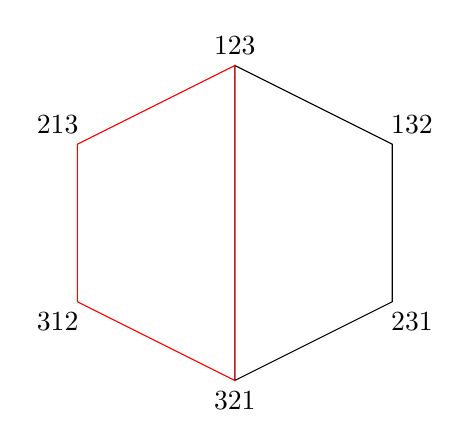
\begin{tikzpicture}
		\draw (0,4) -- (2,3) -- (2,1) -- (0,0) -- cycle;
		\draw [red](0,4) -- (0,0) -- (-2,1) -- (-2,3) -- cycle;
		\node at (0,4.25) {$123$};
		\node at (0,-.25) {$321$};
		\node at (-2.25,3.25) {$213$};
		\node at (2.25,3.25) {$132$};
		\node at (2.25,.75) {$231$};
		\node at (-2.25,.75) {$312$};
	\end{tikzpicture}
	\qquad
	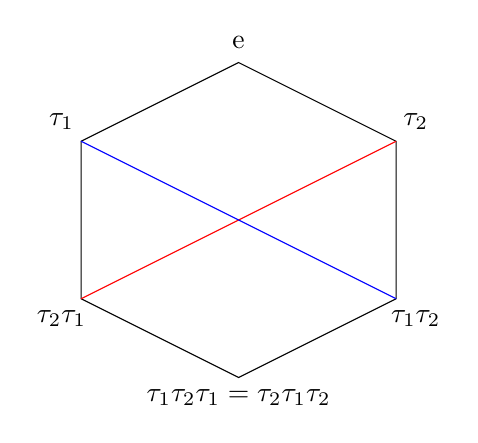
\begin{tikzpicture}
		\draw (0,4) -- (2,3) -- (2,1) -- (0,0) -- (-2,1) -- (-2,3) -- cycle;
		\draw[red] (-2,1) -- (2,3);
		\draw[blue] (-2,3) -- (2,1);
		\node at (0,4.25) {e};
		\node at (0,-.25) {$\tau_{1}\tau_{2}\tau_{1}=\tau_{2}\tau_{1}\tau_{2}$};
		\node at (-2.25,3.25) {$\tau_{1}$};
		\node at (2.25,3.25) {$\tau_{2}$};
		\node at (2.25,.75) {$\tau_{1}\tau_{2}$};
		\node at (-2.25,.75) {$\tau_{2}\tau_{1}$};
	\end{tikzpicture}
	\caption{Left: regular hexagon $\Pi_3$ subdivided into two flag polytopes, neither of which are Bruhat interval polytopes.  Right: Bruhat order of $\Sym(3)$.}
	\label{fig:bruhat}
\end{figure}

\paragraph*{Compression of valuated flag matroids.}


%\hrule
%The 3-term incidence relations on $w_d,w_{d+1}$ are equivalent to the 3-term Pl\"ucker relations of $\mu: {[n+1] \choose d+1}: \RR$ where $\mu(A) = w_d(A-(n+1))$ if $n+1 \in A$ and $\mu(A) = w_{d+1}(A)$ if $n+1 \notin A$.
%\todo{GL: Why should the 3-term incidence relations be equivalent to the full incidence relations? This might be correct, but I do not see an argument here and I also do not see this statement in the literature. JAO: The argument is that the incidence relations are the same as the P\"ucker relations for $\mu$ as defined above. As the 3-term Pl\"ucker relations are enough, provided the support is a matroid, then so are the 3-term Pl\"ucker relations, provided the base matroids form a quotient. But that is the case here since the base matroids are uniform. }

%Since the support of $\mu$ is the whole hypersimplex $\Delta_{(d+1),(n+1)}$, then by \cite{Speyer:2008} \todo{GL: I am not so sure about this reference, where exactly is this stated? I know of a reference by Murota... } they are enough to show that $\mu$ is a valuated matroid and therefor $(w_d,w_{d+1})$ is one-step flag. (Note, the 3-term Pl\"ucker relations are only enough when the support is known to be a matroid \cite[Corollary 5.5]{Rincon:2012} \todo{GL: I could not find this result in the paper. Let's check again. }).

%\todo{JAO: Speyer's classical result says that function ${[n] \choose d}\to \RR$ is a valuated matroid if and only if the corresponding subdivision of the hypersimplex is matroidal \cite[Proposition 2.2]{Speyer:2008}. Felipe generalizes this to $\Delta$-matroids in \cite[Theorem 5.4]{Rincon:2012}. However, in Felipe's theorem, the function is allowed to have $\infty$ entries. So even when restricted to usual matroids ($\Delta$-matroids naturally contain usual matroids) his theorem is still more general than Speyer's; a function ${[n] \choose d}\to \TT$ is a valuated matroid if and only if the support is a matroid and the subdivision is matroidal \cite[Corollary 5.5]{Rincon:2012}.}
%\hrule

%definition of quotient of valuated matroid or tropical incidence relation

%definition of valuated flag matroid

%In the following, $\mu_{M}$ will denote a valuated matroid with underling matroid $M$. 
%Unless otherwise noted, the ground set will be assumed to be $[n]$.
%
%\begin{definition} \label{def:valuated-matroid-quotient}
%Let $\mu_{M}$ and $\mu_{N}$ be valuated matroids of rank $r$ and $s$ respectively, such that $r\leq s$.  
%Then $\mu_{M}$ is a valuated matroid quotient of $\mu_{N}$ if for any $I\in\cB(M)$,$J\in\cB(N)$, and $i\in I\setminus J$, there exitst $j\in J\setminus I$, such that $$\mu_{M}(I)+\mu_{M}(J)\geq \mu_{M}((I\setminus i)\cup j)+ \mu_{N}((J\setminus j)\cup i)$$ 
%\end{definition}

%% \todo{GL: Check which reference to give here. }

%% For a valuated matroid quotient $\mu_{M}$ of $\mu_{N}$, we write $\mu_{M}\twoheadleftarrow \mu_{N}$.
%% When we have a sequence of valuated matroids $\mu=(\mu_{M_{1}},...,\mu_{M_{k}})$ such that $\mu_{M_{i}}\twoheadleftarrow\mu_{M_{j}}$ for all $i<j$, we call $\mu$ a valuated flag matroid. 
%% Note that the sequence of underlying matroids $M=(M_{1},..., M_{k})$ forms a flag matroid.

%% %definition of valuated generalized matroid

%% \todo{GL: It is not clear to me anymore if a full flag of valuated matroids is really the same as a valuated generalized matroid. I am getting mixed up in the definitions and I would have to check more thoroughly. Valuated generalized matroids could still be just a special case of valuated flag matroids...}

%% %definition of compression\\

A height function $w \colon \Sym(n) \to \RR$ is a \emph{valuated permutahedron} if each cell in the induced subdivision of $\Pi_n$ is a subpermutahedron. 
\begin{remark}
	Alternatively, a height function $w \colon \Sym(n) \to \RR$ is a valuated permutahedron if and only if its piecewise-linear extension (i.e. linearly extending over each cell of the subdivision) on the lattice points $\Pi_n \cap \ZZ^{n}$ is an M-convex function.
	In the latter case, it is the supremum over all M-convex functions that agree with $w$ on $\Sym(n)$.   
\end{remark}
It turns out that these are essentially the same as full valuated flags of uniform matroids. 
Let $(\mu_1,\dots,\mu_k)$ be a sequence of valuated matroids with $\rk(\mu_1) < \dots < \rk(\mu_k)$ and underlying matroid $M_1,\dots,M_k$. 
In~\cite{FujishigeHirai:2022}, the \emph{compression} $u \colon \sum_{i=1}^{k}M_i \to\RR$ of $(\mu_1,\dots,\mu_k)$ is defined as the function
\begin{equation*}
	u(x)=\min\biggSetOf{\sum_{i\in[k]}\mu_j(Y_{i})}{x=\sum_{i\in[k]}e_{Y_{i}},\forall i \in [k]:Y_{i}\in \cB(M_i)} \;.
\end{equation*}

When $(\mu_1,\dots,\mu_k)$ in the former definition is a valuated flag matroid, by \cite[Theorem 4.4.2]{BrandtEurZhang:2021}, the cells in the subdivision of $\Pi_n \cap \ZZ^{n}$ induced by $u$ are themselves base polytopes of flag matroids. %\todo{GL: As far as I understand, this rank condition follows from the proof but is actually not stated explicitly; however, to me it seems to be the ingredient, why we don't have interior points in the subdivision. }
Therefore, using \Cref{thm:characterization-flag-base-polytope}, the subdivision is composed of subpermutahedra of $\Pi_n$. 
On the other hand, \cite[Cor.~4.4.5]{BrandtEurZhang:2021} provides us with the converse, namely that such subdivisions arise from the compression of a valuated flag matroid. 

\iffalse


Next we will see that valuated flag matroids are exactly what we need to obtain regular permutahedral subdivisions of base polytopes of flag matroids.

\todo{Dante@Georg: I've rewrote and cited the two theorems below} 
\begin{theorem}\cite[Theorem 4.4.2]{BrandtEurZhang:2021}
	Let $\mu=(\mu_{1},...,\mu_{k})$ be a valuated matroid with underlying flag matroid $M=(M_{1},...,M_{k})$. Regard each $\mu_{i}$ as a weighted points configuration on $\cB(M_{i})$. Then their Minkowski sum $\sum^{k}_{i=1}\mu_{i}$, which is a weight on the base configuration $\cB(\underline{\cM})$, induces a flag matroidal subdivision of $\cB(M)$.
\end{theorem}

\begin{theorem}\cite[Theorem 4.4.3]{BrandtEurZhang:2021}
	Let $M=(M_{1},...,M_{k})$ be a flag matroid on $[n]$, and let $w$ be a weight on the base configuration $\cB(M)$. Suppose the subdivision $\Delta_{w}$ is flag matroidal. Let $\mu_{1},...,\mu_{k}$ be any weights on $\cB(M_{1}),...,\cB(M_{k})$ satisfying $\Delta_{w}=\Delta_{\sum^{k}_{i=1}}\mu_{i}$. Then $\mu_{1},...,\mu_{k}$ are valuated matroids, and $\mu=(\mu_{1},...,\mu_{k})$ is a valuated flag matroid.
\end{theorem}
\todo{Dante @ Georg: I'm looking at the statement of Theorem 4.4.3 in BEZ, and now I see that they use the notation $\cB(\underline{\cM})$ for the domain of $w$. Could this possibly mean that they are restricting only to the vertices? This would clear up the question as to what was happening at the interior lattice points.}

\fi



\begin{theorem}[{\cite{BrandtEurZhang:2021}}]   %[{\cite[Theorem 4.4.3]{BrandtEurZhang:2021}}] 
	\label{thm:equivalenc-permutahedra-flag}
	A height function $w \colon \Sym(n) \to \RR$ is a valuated permutahedron if and only if it is the restriction $u|_{\Sym(n)}$ of the compression of a full flag of valuated uniform matroids. 
\end{theorem}

\iffalse
First consider the restriction $u|_{\Pi_{n}}$. Recall that the vertices of $\Pi_{n}$ are in bijection with flags $B_{1}\subset...\subset B_{n}$, where each $B_{i}\in\cB(M_{i})$. Further, this bijection guarantees a unique representation of each vertex, such that $v=\sum^{n}_{i=1}e_{B_{i}}$ where $(B_{1},...,B_{n})$ is a flag of bases of uniform matroids. Therefore $u|_{\Pi_{n}}(v)=\sum^{n}_{i=1}\mu_{i}(B_{i})$, where $mu_{i}$ is the valuation on $M_{i}$. By \cite[Theorem 4.4.2]{BrandtEurZhang:2021}, this is a valuated permutahedron.

\todo{@Georg: It's not clear to me that the results from 4.4 of BEZ guarantee that every valuated permutahedron is the restriction of the compression of valuated matroids. But I do think I see why the subdivision induced by the valuated permutahedron is also induced by the restriction of a compression to vertices.}

Let $w$ be a valuated permutahedron. Then $w$ induces a permutahedral subdivision of $\Pi_{n}$. By \cite[Theorem 4.4.3]{BrandtEurZhang:2021}, there exists a valuated flag matroid $(\mu_{1},...,\mu_{n})$ such that the Minkowski sum $\sum^{n}_{i=1}\mu_{i}$ induces the same subdivision. Since $w$ is defined on the vertices, \textcolor{red}{(and $\sum^{n}_{i=1}\mu_{i}$ only really makes sense on vertices, but I don't see where BEZ says that)} $\sum^{n}_{i=1}\mu_{i}$ is equal to the restriction of $u$ to points in $\Pi_{n}$ that correspond to nested bases of uniform matroids on $[n]$. In other words, the vertices of $\Pi_{n}$.
\fi

%\todo{GL: Alternative formulation in terms of linear extension of $w$ instead of restriction of $u$?}

%Note that the compression is just the \emph{convolution} of the valuated matroids in the sense of \todo{GL: Add ref. }.

%% \hrule

%% \begin{definition}
	%% Let $f:2^{[n]}\to\RR$ be submodular, and $g$ defined on the same domain be supermodular, such that $f(\emptyset)=g(\emptyset)=0$ and $$f(X)-g(Y)\geq f(X\setminus Y)-g(Y\setminus X)$$ for all $X,Y\subset [n]$. Then the polyhedron $$P(f,g)=\{x\in\RR^{n}|\forall X\in 2^{[n]}:g(X)\leq \sum^{n}_{i=1}x_{i}\leq f(X)\}$$ is called a {\it generalized polymatroid}.
	%% \end{definition}
%% Let $P(f,g)$ be a generalized polymatroid with vertices in $\{0,1\}^{n}$. Then we can identify the vertices of $P(f,g)$ with a subset $\mathcal{G}=\{B\in 2^{[n]}:e_{B}\in V(P(f,g))\}$. Then $\mathcal{G}$ is a {\it generalized matroid}.
%% \begin{definition}
	%% An $M^{\sharp}$ convex function is a polyhedral convex function $f:\RR^{n}\to\RR\cup\{\infty\}$ satisfying:
	%% \begin{itemize}
		%% \item The effective domain $\text{dom}(f)=\{x\in\RR^{n}:f(x)<\infty\}$ is a generalized polymatroid
		%% \item Every linearity domain of $f$ is a generalized polymatroid
		%% \end{itemize}
	%% where the linearity domain of $f$ is $\text{Argmin}(f-h)$, $h\in\left(\RR^{n}\right)^{*}$ is a linear functional. 
	%% \end{definition}
%% \begin{definition}
	%% Let $f:\ZZ^{n}\to\ZZ\cup\{\infty\}$ be an $M^{\sharp}$ convex function.
	%% If the effective domain $\text{dom}(f)=\{0,1\}^{n}$, then we call $f$ a valuated generalized matroid. 
	%% \end{definition}

%% Let $f:\ZZ^{n}\to\RR\cup\{\infty\}$ be $M^{\sharp}$ convex, where the effective domain $\text{dom}(f)=P(f^{*},g^{*})$ is bounded full dimensional. In otherwords, $f^{*}$ and $g^{*}$ are submodular and supermodular functions respectively such that $\infty>f^{*}(E)>g^{*}(E)$.

%% \begin{definition}
	%% Let $I_{f}=\{\alpha\in\ZZ:f^{*}(E)\geq\alpha\geq g^{*}(E)\}$.
	%% For each $\alpha\in I_{f}$, define the {\it $\alpha$-section} of $f$ to be the function $f_{\alpha}:\ZZ^{n}\to\RR\cup\{\infty\}$ such that
	%%  \begin{center}
		%% $f_{\alpha}(x)=\begin{cases}
			%% f(x) &\text{ if } \sum_{i\in[n]}x_{i}=\alpha\\
			%% \infty &\text{ otherwise}\\
			%% \end{cases}$
		%% \end{center}
	%% \end{definition}
%% \begin{definition}
	%% For an $M^{\sharp}$ convex function $f:\ZZ^{n}\to\RR\cup\{\infty\}$ whose effective domain is bounded and full dimensional, we define the the {\it compression} of $f$ to be the function $\hat{f}:\ZZ^{n}\to\RR$ such that $$\hat{f}(x)=\text{min}\left\{\sum_{\alpha\in I_{f}}f_{\alpha}(y_{\alpha})\big{|}x=\sum_{\alpha\in I_{f}}y_{\alpha},\forall \alpha\in I_{f}:y_{\alpha}\in\ZZ^{n}\right\}$$
	%% \end{definition}
%% \begin{definition}
	%% Let $f:\ZZ^{n}\to\ZZ\cup\{\infty\}$ be an $M^{\sharp}$ convex function with effective domain $\dom(f)=\{0,1\}^{n}$. Then we say $f$ is a {\it valuated generalized matroid}.
	%% \end{definition}

%% For $A\subset [n]$, we denote $f(A)=f\left(e_{A}\right)$. With this in mind, we define the compression of valuated generalized matroids as follows.


%% %summarize results in Section 4.4 in BEZ
%% \todo{Dante: I feel like we could come up with notation to make for the transition between the Compression material and the BEZ material smoother}





%\todo{GL: I am currently still trying to figure out, to which extent the next claim is already given in \cite{MurotaShioura:2018}. -- So as we discussed it might be that the following statement does not need the condition of being downwards closed really because we have a function on the full support. }
\paragraph*{Incidence relations imply Pl\"ucker relations}

Now, we deal with the interplay of the valuated matroids in a flag.
For (non-tropical) Pl\"ucker vectors, the implication of the Pl\"ucker relation from the incidence relation occurred in~\cite{JellMarkwigRinconSchroter:2003.02660}.
On the combinatorial level, this was studied in the context of \enquote{M$^{\natural}$-convex set functions}; cf.\ \cite{MurotaShioura:2018}.
Indeed, imposing supermodularity among the constituents of a valuated flag matroid gives rise to an M$^{\natural}$-convex set function. 

\begin{theorem} 
  \label{thm:1step}
  Let $\nu : \binom{[n]}{d} \to \RR$ and $\mu : \binom{[n]}{d+1} \to \RR$ be any two functions satisfying the tropical incidence relations \eqref{eq:3-term-incidence}. 
  Then $\mu$ and $\nu$ are valuated matroids.
\end{theorem}
\begin{proof}
	We show that $\mu$ satisfies the 3-term Pl\"ucker relations: for all $S\in\binom{[n]}{d-1}$ and $i,j,k,l \in [n]\backslash S$ the minimum in $\min(\mu(Sij) + \mu(Skl),\mu(Sik) + \mu(Sjl),\mu(Sil) + \mu(Sjk))$
	is attained at least twice.
	For a contradiction, suppose there is a set $S$ and $i,j,k,l \in [n]\backslash S$ with
	\begin{equation} \label{eq:violated-twice-min}
		\mu(Sij) + \mu(Skl) < \mu(Sik) + \mu(Sjl) \quad \text{and} \quad \mu(Sij) + \mu(Skl) < \mu(Sil) + \mu(Sjk) \, .
	\end{equation}
	
	Let $\xi = \nu(Si) e_i + \nu(Sj) e_j + \nu(Sk) e_k + \nu(Sl) e_l$.
	Defining $\mu'$ with $\mu'(T) = \mu(T) - \langle\xi,e_T\rangle$ for all $T \in \binom{[n]}{d+1}$ and defining $\nu'$ by the same translation from $\nu$, the pair $(\mu,\nu)$ is a valuated matroid quotient if and only if $(\mu',\nu')$ is a quotient.
	Hence, we can assume that $\nu(Si) = \nu(Sj) =\nu(Sk) = \nu(Sl) = 0$. 
	With this, \eqref{eq:3-term-incidence} yields that the minima in $\min(\mu(Sij),\mu(Sik),\mu(Sjk))$, $\min(\mu(Sik),\mu(Sil),\mu(Skl))$, $\min(\mu(Sik),\mu(Sil),\mu(Skl))$, are attained twice.
	 By \eqref{eq:violated-twice-min}, $\min(\mu(Sij),\mu(Skl)) \leq \max(\mu(Sik),\mu(Sjl),\mu(Sil),\mu(Sjk))$, so we can assume that $\mu(Sij) < \mu(Sik)$.
	
	Combining the two observations yields $\mu(Sij) = \mu(Sjk)$.
	From the second inequality in~\eqref{eq:violated-twice-min}, we get $\mu(Skl) < \mu(Sil)$.
	By the minimum condition, we have $\mu(Skl) = \mu(Sik)$. 
	From the first inequality in~\eqref{eq:violated-twice-min}, we get $\mu(Sij) < \mu(Sjl)$.
	Again by the minimum condition, $\mu(Sij) = \mu(Sil)$. 
	With the above, this yields $\mu(Sij) = \mu(Sil) > \mu(Skl) = \mu(Sik)$, which contradicts the original assumption. 
	Hence $\mu$ satisfies all 3-term Pl\"ucker relations and therefore it is a valuated matroid.
	By duality, $\nu$ must also be a valuated matroid.
\end{proof}


\section{Regular permutahedral subdivisions}

Based on the structure of the permutahedron, we derive conditions for a regular subdivision to be permutahedral: 
a height function induces a permutahedral subdivision of $\Pi_n$ if and only if it does so in the 2-skeleton of $\Pi_n$.
% Explicitly, the 2-dimensional faces of $\Pi_n$ are hexagons and squares, see \Cref{sec:geometry-regular-permutahedron}.
% A permutahedral subdivision cannot introduce diagonals in the squares and it can only have long diagonals in hexagons.

To this end consider an arbitrary polytope $P$ with vertex-edge graph $\Gamma=(V,E)$.
We duplicate each edge, equipped with two opposite orientations; this turns $\Gamma$ into a directed graph, which we denote $\Gamma^\pm=(V,E^\pm)$.
Now any function $f:V\to\RR$ defined on the vertices yields a function $g:E^\pm\to\RR$ on the directed edges by letting
\begin{equation}\label{eq:potential}
  g(v,w) = f(v)-f(w) \qquad \text{for distinct } v,w\in V \; ,
\end{equation}
where $g(w,v)=-g(v,w)$.
The key observation is that $f$ can be recovered from $g$ under mild conditions.
We assume $n:=\dim P\geq 2$, whence $\partial P\approx\Sph^{n-1}$ is simply connected.
\begin{proposition}\label{prop:potential}
  Let $g:E^\pm\to\RR$ be a function on the directed edges of $P$ which satisfies $\sum_{i=1}^{k} g(v_i,v_{i+1})=0$ for every $2$-face of $P$ with vertices $v_1,v_2,\dots,v_{k+1}=v_1$ (labeled cyclically).
  Then there is a unique function $f:V\to\RR$ on the vertices with \eqref{eq:potential} and $f(s)=f_0$ for any fixed $s\in V$ and $f_0\in\RR$.
\end{proposition}
\begin{proof}
  Pick a directed spanning tree $T$ of $\Gamma^\pm$ rooted at $s$, and define a function $f:V\to\RR$ by inductively setting $f(s)=f_0$ and $f(v) = g(v,w) + f(w)$ along the directed edges of $T$.
  We need to show that $f$ satisfies $f(v)-f(w)=g(v,w)$ for distinct vertices $v,w$.
  To this end it suffices to prove that $h(c):=\sum_{i=1}^{\ell} g(w_i,w_{i+1})=0$ holds for any directed cycle $c=(w_1,w_2,\dots,w_\ell,w_{\ell+1}=w_1)$ in $\Gamma$.
  The boundary complex $\partial P$ is a polytopal complex homeomorphic to $\Sph^{n-1}$.
  A combinatorial procedure for computing the fundamental group of a polytopal complex is given in \cite[\S44]{SeifertThrelfall} (where this is proved for simplicial complexes).
  This has the following consequences.
  First, any path in $\partial P$ is homotopic to a path in $\Gamma$.
  Second, due to $n\geq 2$, the boundary $\partial P \approx \Sph^{n-1}$ is simply connected, and thus every closed path in $\Gamma$ can be contracted to a constant path within the $2$-skeleton of $P$.
  In this way, up to homotopy, the cycle $c$ can be contracted combinatorially in the following sense: there is a sequence of cycles $c_1, c_2, \dots, c_m$ in $\Gamma$ such that $c_1=c$, the cycle  $c_m$ is trivial (without any edges), and the symmetric difference between the edges in $c_i$ and $c_{i+1}$ forms a $2$-face.
  Now the assumption on $g$ gives $0=h(c_m)=h(c_{m-1})=\dots=h(c_0)=h(c)$, as we wanted to show.
  A similar argument yields the uniqueness of $f$.
\end{proof}
% Keep this comment, even if it is not strictly necessary (which is why we delete it from the text).
% The above argument is similar to the proof of \cite[Theorem~8]{Joswig:2002}; see also \cite[\S8.2]{Schrijver03:CO_A}.
Before we will apply this statement to the hypersimplex, we need to relate functions on the permutahedron and on the hypersimplex. 
To this end let $G^\pm_{\Pi}(n)$ be the directed vertex-edge graph of $\Pi_n$ as above.
Similarly, let $G^\pm_\Delta(d,n)$ be a directed version of the vertex-edge graph of the hypersimplex $\Delta(d,n)$.
Recall that each edge of $\Pi_n$ gives rise to a pair $(A,B)$ of equicardinal subsets of $[n]$ with $|A \triangle B| = 2$, and that each edge of $\Delta(d,n)$ corresponds to a pair $(A,B)$ of d-subsets of $[n]$ with $|A \triangle B| = 2$. 

\begin{lemma} \label{lem:squares-function}
  Let $g$ be a function on the directed edges of $G^\pm_{\Pi}(n)$ such that, on each $2$-face of $\Pi_n$ which is a square, parallel directed edges attain the same $g$-value.
  Then this yields a function $g'$ on the directed edges of $\bigcup_{d=0}^{n} G^\pm_{\Delta}(d,n)$ such that $g'(A,B) = g(e)$ for all equicardinal subsets of $[n]$ with $|A \triangle B| = 2$ and all edges $e$ of $\Pi_n$ corresponding to $(A,B)$. 
\end{lemma}
\begin{proof}
  Let $(A,B)$ be a pair of equicardinal subsets of $[n]$ with $|A \triangle B| = 2$.
  By \Cref{faces-permutahedron}, the vertices given by the full flags extending $(A \cap B, A \cup B)$ form a face isomorphic with $\Pi_{|A \cap B|} \times \Pi_{2} \times \Pi_{n - |A \cup B|}$.
  %In particular, any two of these edges are connected by a sequence of edges on this face, where each edge gives rise to a square by taking the product with an edge corresponding to $(A,B)$.
	In particular, any two of these edges are connected by a sequence of squares on this face, where each square is composed by a pair of parallel edges corresponding to $(A,B)$ and are adjacent to each other in this sequence along these edges.
  By the condition on the squares, all the edges in $G^\pm_{\Pi}(n)$ corresponding to $(A,B)$ have the same $g$-value.
  So we take that number to define $g'$ on the arc of $G^\pm_{\Delta}(d,n)$ corresponding to $(A,B)$, where $d = |A| = |B|$.
\end{proof}

%% \textbf{Lemma A} describing the structure of the set of all square faces on the permutahedron which have the same edge label on two opposite edges (the label is the pair of sets $A,B$ of the same cardinality with $|A \triangle B| = 2$ by which the two complete flags of its vertices differ).
%% Then deduce that any function defined on the vertices of the permutahedron defines a function on all pairs if it fulfills the square condition.

%% \textbf{Lemma B} 3-term incidence relations

\begin{theorem}
	\label{thm:regular-2-skeleton}
	A height function $w \colon \Sym(n) \to \RR$ induces a permutahedral subdivision if and only if it induces a permutahedral subdivision of the 2-skeleton of $\Pi_n$. That is:
	\begin{enumerate}[leftmargin=*, widest=XXXX]
		\item[(HEX)] for every hexagon $abcdef$ (labeled cyclically) in the 2-skeleton of $\Pi_n$, we have
		\begin{enumerate}
			\item[(HXE)] $w(a)+w(c)+w(e) = w(b)+w(d)+w(f)$, 
			\item[(HXM)] the maximum in $\max(w(a)+w(d), w(b)+w(e), w(c)+w(f))$ is attained twice;
		\end{enumerate}
		\item[(SQR)] for every square face $abcd$ of $\Pi_n$ (labeled cyclically): $w(a)+w(c) = w(b)+w(d)$.
	\end{enumerate}
\end{theorem}

\begin{proof}
	A subdivision of a polytope defines a subdivision on each face.
	Therefore, as each cell in the subdivision is a subpermutahedron, the 2-faces are also subdivided into subpermutahedra. 
	Since squares cannot be subdivided any further, the second condition follows.
	To show the first condition, observe that at least four cyclically consecutive vertices have to lie in the same hyperplane, the other two on or above. 
	By relabeling and subtracting a linear form, we can assume that $w(a) = w(b) = w(c) = w(d) = 0$ and that $w(e) = w(f) \geq 0$. 
	This implies that the conditions on the $2$-skeleton are necessary.
	
	For the converse, suppose that $w$ satisfies the conditions (HEX) and (SQR).
	We will show that $w$ can be decomposed into a flag of valuated matroids $(g_1,\dots,g_n)$ such that $w$ is the result of their compression. 
	Then, by \Cref{thm:equivalenc-permutahedra-flag}, $w$ is a valuated permutahedron.
	
	On each directed edge $(a,b)$ in $G^\pm_\Pi(n)$, we let $h'(a,b) = w(a) - w(b)$ as above.
	Using (SQR), by \Cref{lem:squares-function}, this defines a function $h_d$ on the directed edges of $G^\pm_{\Delta}(d,n)$ for any $d$.
	We fix an arbitrary vertex $u$ of $\Pi_n$, which corresponds to a full flag $\mathcal{G} = (G_1, \dots, G_n)$ in $[n]$.
	Recall that a hexagon corresponds to the flags extending $(S,S {} ijk)$ for some $S$ and $i,j,k \in [n] \setminus S$.
	With this notation the condition (HXE) amounts to
	\[
	h(S {} i, S {} j) + h(S {} j, S {} k) + h(S {} k, S {} i) =
	h(S {} ij, S {} jk) + h(S {} jk, S {} ik) + h(S {} ik, S {} ij) = 0 \,.
	\]
	It follows that $h$ sums to zero along each oriented $2$-face of $\Delta(d,n)$ (i.e., a triangle).
        Thus \Cref{prop:potential} yields a function $g$ on the vertices of $\Delta(d,n)$ with $\sum_{d=1}^{n}g(G_d) = w(u)$.
	
	Let $v$ be an arbitrary vertex of $\Pi_n$, which corresponds to a full flag $\cF = (F_1, \dots, F_n)$ in $[n]$.
	As a path from $u$ to $v$ decomposes into paths from $G_d$ to $F_d$ on $\Delta(d,n)$, we have $w(v)=\sum_{d = 1}^{n} g_d(F_d)$. 
	For a hexagon face described by the flags extending $(S,S {} ijk)$ with some $S \subset [n]$ and $i,j,k \in [n] \setminus S$, the sum representation of $w$ agrees in all terms with $d \leq |S|$ and $d \geq |S| + 3$.
	Hence, by (HXM), the maximum is attained at least twice in 
	\begin{equation*}
		\begin{aligned}
			\max\bigl(\, g(S {} i) + g(S {} ij) + g(S {} k) + g(S {} jk),\; & g(S {} j) + g(S {} jk) + g(S {} i) + g(S {} ik), \\
			&g(S {} k) + g(S {} ik) + g(S {} j) + g(S {} ij) \, \bigr) \;.
		\end{aligned}
	\end{equation*}
	
	Subtracting $g(S {} i) + g(S {} j) + g(S {} k) + g(S {} ij) + g(S {} ik) + g(S {} jk)$ and multiplying by $-1$ yields that $\min(g(S {} j) + g(S {} ik), g(S {} k) + g(S {} ij), g(S {} i) + g(S {} jk))$
	attains the minimum twice.
	This is the 3-term incidence relation.
	Summarizing, we have proven that $(g_1,\dots,g_n)$ satisfy the 1-step Pl\"ucker relations.
	By \Cref{thm:1step} all of the $g_d$ are valuated matroids and so $(g_1,\dots,g_n)$ is a valuated flag matroid.
\end{proof}


% \todo{JAO: I believe that there is a chance that this generalizes to any function whose support is a subpermuthaedron. We wold need to add the square condition for the trapezoids (half hexagons) that appear. -- GL: Maybe put as conjecture.  }

\section{Total positivity} 
The positive tropical Grassmannian $\TGr^+(d,n)$ is the tropicalization of the positive part of the Grassmannian $\Gr^+(d,n)$ consisting of linear spaces over the reals with all Pl\"ucker coordinates positive; see \cite{SpeyerWilliams:2005,SpeyerWilliams:2021,ArkaniHamedLamSpradlin:2021}.
Following~\cite[Equation~(1.1)]{ArkaniHamedLamSpradlin:2021}, a valuated matroid $v$ is \emph{positive} if it fulfills the three-term positive tropical Pl\"ucker relations; i.e., for every $S$ and $i < j < k < l$ not in $S$, we have
\begin{equation} \tag{3TPR+} \label{eq:positivepluecker}
	v(Sik) + v(Sjl) = \min(v(Sij)+v(Skl), v(Sil)+v(Sjk)) \;.
\end{equation}

Similarly, the positive part of the (full) flag variety can be defined as the space of full flags $\cL=(L_1, \dots, L_n)$ where $L_d \in \Gr^+(d,n)$.
Let us formulate an \enquote{untropicalized} analog of one of the directions of \Cref{thm:regular-2-skeleton}.
The Pl\"ucker coordinates of a linear space $L_d\subseteq \KK^n $ over some field $\KK$ can be organized into a polynomial: 
\[
f_{L_d}(x) = \sum_{B\in \binom{[n]}{d}} p_B \prod_{i\in B} x_i \in \KK[x_1,\dots,x_n] \;,
\]
whose support is the base polytope of the matroid $M(L_d)$.
As a side remark, note that in~\cite{Purbhoo:2018} such a polynomial was shown to encode a totally nonnegative linear space if and only if it is stable. 
Given the flag $\cL$, the coefficients of these polynomials satisfy
\begin{equation} \label{eq:classical-incidence}
p_{Si}p_{Sjk} - p_{Sj}p_{Sik} + p_{Sk}p_{Sij} = 0 \;.
\end{equation}
for all $S\subseteq [n]$ and $i<j<k$ not in $S$.
To give an analog of \eqref{eq:positivepluecker}, we work our way from the equation above to reach the condition (HXM).

The product $f_{L_1}\cdots f_{L_n}$ is a polynomial whose support is the flag matroid base polytope $M(L_1) + \dots+ M(L_n)$. 
Suppose this polytope is the regular permutahedron $\Pi_n$ and let $q_\sigma$ be the coefficient of $x_1^{\sigma(1)}\cdots x_n^{\sigma(n)}$ in $f_{L_1}\cdots f_{L_n}$.
Hence, for $n=3$, we have that $q_{\sigma} = p_{\sigma^{-1}(3)}p_{\sigma^{-1}(2)\sigma^{-1}(3)}p_{\sigma^{-1}(1)\sigma^{-1}(2)\sigma^{-1}(3)}$ yielding with~\eqref{eq:classical-incidence} then 
\[
\begin{aligned}
	q_{(321)}q_{(123)}&q_{(231)}q_{(213)} - q_{(231)}q_{(213)}q_{(312)}q_{(132)} +  q_{(312)}q_{(132)}q_{(321)}q_{(123)} \\
	&= p_1p_2p_3p_{12}p_{13}p_{23}p_{123}^4 \left(p_{12}p_3-p_{13}p_2+p_{23}p_1 \right) = 0 \;.
\end{aligned}
\]
Notice as well that $p_1p_2p_3p_{12}p_{13}p_{23} = q_{(123)}q_{(231)}q_{(312)}=q_{(321)}q_{(213)}q_{(132)}$.
From here we can deduce the following relations that must be satisfied for any $n$:
\begin{itemize}
	\item For every hexagonal face $abcdef$ (labeled cyclically) of $\Pi_n$ we have $q_aq_cq_e = q_bq_dq_f$ and $q_bq_cq_eq_f -q_aq_cq_bq_f+ q_aq_bq_dq_e = 0$. By \cite[Section 4.3]{TsukermanWilliams} hexagons are Bruhat interval polytopes, and the negative term  $q_aq_cq_bq_f$ is the one not containing the lowest and largest elements of this interval.
	\item For every square face $abcd$ (labeled cyclically) of $\Pi_n$ we have $q_aq_c = q_bq_d$.
\end{itemize}

%Observing these relation for $\Pi_3$ we have that 
%\begin{align*}
%p_{12}p_3-p_{13}p_2+p_{23}p_1 &= p_1p_2p_3p_{12}p_{13}p_{23}\left( \frac{1}{p_1p_2p_{13}p_{23}} -\frac{1}{p_1p_3p_{12}p_{23}} +\frac{1}{p_2p_3p_{12}p_{13}} \right) \\
%&= p_1p_2p_3p_{12}p_{13}p_{23} \left(\frac{1}{q_{(312)}q_{(132)}} -  \frac{1}{q_{(321)}q_{(123)}} + \frac{1}{q_{(231)}q_{(213)}} \right).
%\end{align*}
%
%Similarly, any hexagonal face of $\Pi_n$ can be reduced to this case.

This suggests the following positivity condition for the tropicalization of the positive part of the flag variety; see \Cref{ex:bruhat}: 
\begin{enumerate}[leftmargin=*, widest=XXXXX]
	\item[(HXM+)] \label{eq:positiveflag} For every (cyclically labeled) hexagon $abcdef$ of $\Pi_n$, where $b$ is the lowest permutation in the Bruhat order, $w(b)+w(e) = \max(w(a)+w(d), w(c)+w(f))$.
\end{enumerate}

%\begin{equation} \tag{HXM+}
%w(b)+w(e) = \max(w(a)+w(d), w(c)+w(f)).	
%
%\end{equation}
%\todo{GL: In the following, this equation is referred to as the collection of all requirements on $w$ not only the $\max$-attainment -- we have to be careful here. }

We will need the following positivity adaptation of \Cref{thm:1step}:
\begin{lemma}\label{lemma:1step_positive}
	Let $\nu : \binom{[n]}{d} \to \RR$ and $\mu : \binom{[n]}{d+1} \to \RR$ be any two functions such that for every $S\in \binom{[n]}{d-1}$ and $i<j<k \notin S$, 
	\[
	\nu(Sj)+\mu(Sik) = \min(\nu(Si)+\mu(Sjk),\nu(Sk)+\mu(Sij)) \;.
	\]
	Then $\nu\in \TGr^+(d,n)$ and $\mu \in  \TGr^+(d+1,n)$.
\end{lemma}
\begin{proof}
	By \Cref{thm:1step} we know already that $\nu$ and $\mu$ are valuated matroids. 
	Again we can do a translation to assume $\nu(Si)=\nu(Sj)=\nu(Sk)=\nu(Sl)=0$.
	Suppose $\mu$ does not satisfy \eqref{eq:positivepluecker}.
	Then w.l.o.g.~$\mu(Sik)+\mu(Sjl)>\mu(Sij)+\mu(Skl)$. 
	However, by the assumption of the lemma, $\mu(Sik)\leq \mu(Sij)$ and $\mu(Sjl) \leq \mu(Skl)$, a contradiction. 
\end{proof}

\begin{theorem}\label{thm:positivity}
  Let $u \colon \Sym(n) \to \RR$.
  Then the following are equivalent:
	\begin{enumerate}
		\item The function $u$ is the compression of a valuated flag $(w_1,\dots, w_n)$ which can be realized by a totally positive flag of linear spaces.
		\item All polytopes in the subdivision induced by $w$ are Bruhat interval polytopes.
		\item The function $u$ satisfies conditions (HXE) and (SQR) from \Cref{thm:regular-2-skeleton} as well as (HXM+).
	\end{enumerate}
\end{theorem}

\begin{proof}
	\enquote{$(1)\rightarrow (2)$}.
	Consider a totally positive flag $\cL=(L_1,\dots, L_n)$ that realizes $(w_1,\dots,w_n)$, e.g., over the field of Puiseux series, or a suitable extension for irrational coefficients; see \cite[\S2.6]{ETC}.
	For any polytope $P$ in the subdivision induced by $w$, we can obtain a flag $\tilde{\cL} =(\tilde{L}_1,\dots,\tilde{L}_n)$ that realizes the flag matroid corresponding to $P$ by taking a suitable rescaling of the flag $\cL$ and taking its quotient to the residue field, which is a subfield of $\RR$. 
	By construction, $\tilde{\cL}$ is in the totally non-negative part; yet some Pl\"ucker coordinates may vanish in the quotient. 
	Due to \Cref{prop:bruhat}, $P$ is a Bruhat polytope.
	
	\enquote{$(2) \rightarrow (3)$}.
	By \Cref{thm:regular-2-skeleton} and \Cref{prop:bruhat}, if the subdivision consists of Bruhat polytopes then (HXE) and (SQR) are satisfied.
	Suppose (HXM+) fails, so there is a hexagon where the maximum is not attained by the diagonal connecting the lowest and largest terms in the Bruhat order. 
	Then this diagonal appears in the subdivision and it is not a Bruhat interval polytope; see Figure~\ref{fig:bruhat}. 
	
	\enquote{$(3) \rightarrow (1)$}.
	First notice that by \Cref{thm:regular-2-skeleton} the function $u$ is the compression of the valuated flag matroid $(w_1,\dots, w_n)$. 
	Now consider the valuated matroid $\mu$ on the uniform matroid $U_{n,2n}$ given by $\mu(B) = w_{|B\cap[n]|}(B\cap[n])$; this construction appears, e.g., in \cite{MurotaShioura-conjugate:2018}. 
	That $\mu$ is actually a valuated matroid depends on the right choice of $w_d$, which vary up to adding a constant. 
	To see this and that, moreover, $\mu \in \TGr^+(n,2n)$ we look at the 3-term Pl\"ucker relations \eqref{eq:positivepluecker}. 
	These are given by a set $S\in \binom{[2n]}{d-2}$ and $i,j,k,l \notin S$ and suppose $i< j<k< l$.
	We have the following cases:
	% Such a valuated matroid exists due to (TODO cite Lemma 7.4 in {\url{https://www.renatoppl.com/papers/gs-survey-aug-14.pdf}}). 
	% \todo{JAO: TODO cite Lemma 7.4 in {\url{https://www.renatoppl.com/papers/gs-survey-aug-14.pdf}}. GL: Maybe this reference~\cite{MurotaShioura-conjugate:2018}}
	\begin{itemize}
		\item $|\{i,j,k,l\}\cap[n]| \le 1$. In this case all terms in the Pl\"ucker relation are equal.
		\item $|\{i,j,k,l\}\cap[n]| = 2$. Assuming $i,j \in [n]$, we have that $\mu(Sik) +\mu(Sjl)= \mu(Sil)+\mu(Sjk) = w_{m+1}(Ti) + w_{m+1}(Tj)$ and $\mu(Sij)+\mu(Skl) = w_{m+2}(Tij)+w_{m}(T)$, for $T = S \cap [n]$ and $m = |T|$.
			Here is where we need to ensure supermodularity, i.e. $w_{m+2}(Tij)+w_{m}(T) \ge w_{m+1}(Ti) + w_{m+1}(Tj)$. 
      Since we have the freedom to choose each $w_d$ up to addition of a constant, we can achieve this by adding to each $w_d$ a suitably scaled convex function on $d$. %\todo{GL: This is still super vague and should be made more precise. }
		  As such a transformation preserves the compression $u$, we can ensure that $\mu(Sik) +\mu(Sjl)$ does attain the minimum.
                  
		\item $|\{i,j,k,l\}\cap[n]| = 3$. The positive Pl\"ucker relation here is equivalent to the positive 3-term incidence relation between $w_{|S\cap[n]|+1}$ and $w_{|S\cap[n]|+2}$.
		The proof of \Cref{thm:regular-2-skeleton} shows that the 3-term incidence relations are already implied by (HXM). % which are weaker than (HXM+).
		Further, (HXM+) strengthens this to imply \eqref{eq:positivepluecker}, since the terms of different sign agree under the correspondence of this implication, as seen in the discussion preceding the formulation of (HXM+).
		%in the incidence relation corresponds to the term with the lowest and largest elements of the Bruhat interval. 
		%\todo{GL: Which explanation does this refer to? JAO: The entire page preceding Lemma 11 -- GL: I still don't see how the untropicalized relations play a role here. Shouldn't this just be from the tropical version directly? }
		\item $|\{i,j,k,l\}\cap[n]| = 4$. In this case the Pl\"ucker relation is equivalent to a Pl\"ucker relation in $w_{|S\cap[n]|+2}$.
		By \Cref{lemma:1step_positive}, the positive variation of this relation follows from the last case. 
	\end{itemize}
	%  \todo{GL: The first part of this proof of (3) to (1) should be an extra lemma?!}

        It was recently shown in~\cite{SpeyerWilliams:2021,ArkaniHamedLamSpradlin:2021} that the positive Grassmannian equals the positive Dressian.
        Hence, $\mu$ is realizable by some totally positive subspace $L\in \Gr^+(n,2n)$. Consider $\pi$ to be the projection to the first $n$ coordinates and let $L_d= \pi(L\cap \{x_{n+d+1}=\dots = x_{2n} = 0\})$. The tropicalization of $L_d$ corresponds to the valuated matroid 
	\[
	\mu\backslash \{n+1,\dots, n+d\} / \{n+d+1,\dots, 2n\} = w_d \;.
	\]
	We have $L_1\subset \dots \subset L_n$, all of which are positive.
        So $(w_1,\dots,w_d)$ is in the positive tropical flag variety.					
\end{proof}

% mode: latex
% mode: TeX-PDF
% mode: reftex
% mode: font-lock
% fill-column: 120
% buffer-file-coding-system:utf-8-unix
% End: 
